\documentclass[main.tex]{subfiles}

\begin{document}

\captionsetup[figure]{labelfont={},labelformat={default},labelsep=period,name={Рис.}}

\begin{center}
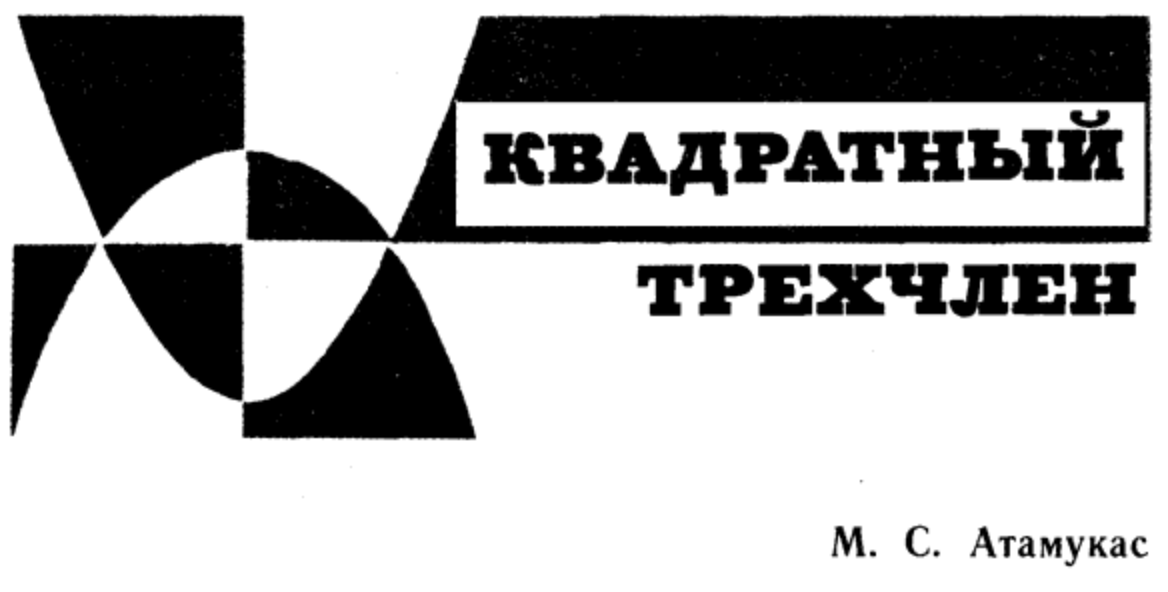
\includegraphics[width=1\textwidth]{picture}
\end{center}


Квадратным трехчленом называют многочлен второй степени общего вида

\begin{center}
$ax^{2} + bx + c, \quad a \ne 0$
\end{center}

На вступительных экзаменах по математике задачи, прямо или косвенно связанные с квадратным трехчленом, предлагаются довольно часто. Да это и не удивительно - в школьной программе уделяется много места и времени изучению квадратного уравнения

\begin{center}
$ax^{2} + bx + c = 0$
\end{center}

\noindent выяснению свойств квадратичной функции

\begin{center}
$y = ax^{2} + bx + c$
\end{center}

\noindent Эта функция встречается и в физике; например, при описании движения материальной точки, брошенной наклонно к горизонту.

Школьники, конечно, хорошо знают все формулы, относящиеся к квадратному трехчлену, умеют они и изобразить график квадратичной функции - параболу. Однако, когда речь идет о решении конкретной задачи, большинство пытается действовать чисто аналитически, привлекая лишь формулы. Между тем очень часто использование геометрических соображений позволяет получить ответ проще и быстрее. Мы покажем на нескольких примерах, как важно бывает при решении задач мыслить одновременно и на алгебраическом, и на геометрическом языках.

Для того, чтобы проверить насколько хорошо вы знакомы со свойствам квадратного трехчлена, рассмотрим сперва такую задачу (она предлагалась на устных экзаменах в МГУ).

\begin{figure}[!htb]
   \begin{minipage}{0.48\textwidth}
     \centering
     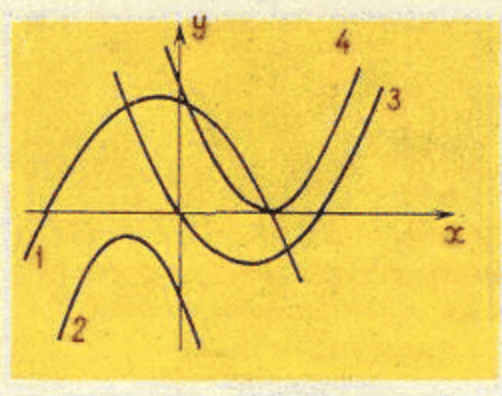
\includegraphics[width=.7\linewidth]{fig1}
     \caption{}\label{Fig:Data1}
   \end{minipage}\hfill
   \begin{minipage}{0.48\textwidth}
     \centering
     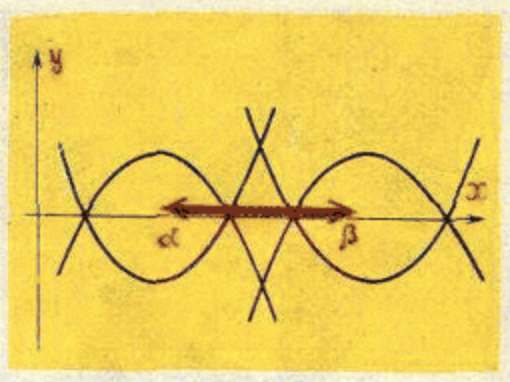
\includegraphics[width=.7\linewidth]{fig2}
     \caption{}\label{Fig:Data2}
   \end{minipage}
\end{figure}

1. \textit{На рисунке \ref{fig:fig1} изображено несколько графиков квадратных трехчленов. Рисунок приблизительный, масштаб не указан. Для каждой из этих парабол определить знаки соответствующих коэффициентов a, b, и c.}

Возьмем, например, параболу 4; она является графиком некоторой квадратичной функции

\begin{center}
$f (x) = ax^{2} + bx + c$.
\end{center}

\noindent Так как ветви этой параболы направлены вверх, то коэффициент a>0. (Докажите! Многие поступавшие объясняли это так: ``В учебнике доказывается, что если a>0, то парабола направлена вверх''. Убедительно ли такое объяснение?). Далее, коэффициент c равен значению функции y в точке x=0, то есть c=f (0). Из рисунка видно, что парабола 4 пересекает положительную полуось ординат, а потому c>0. Абсцисса вершины параболы равна $-\frac{b}{2a}$; из рисунка ясно, что она положительна. Мы уже знаем, что a>0, и, следовательно b<0;

Ответ: a>0, b<0, c>0.

Остальные случаи, представленные на рисунке \ref{fig:fig1}, читатели могут разобрать самостоятельно.

Во многих задачах необходимо выяснить поведение квадратичной функции $f (x) = ax^{2} + bx + c$ на заданном промежутке $(\alpha, \beta)$, описать расположение корней этого трехчлена относительно фиксированной точки $x=y$ оси абсцисс и т. д. В этих задачах геометрический язык делает рассуждения простыми и наглядными (и притом вполне строгими!).

\end{document}